%\documentclass[fleqn]{book}
\documentclass[11pt]{amsbook}

\usepackage[turkish]{babel}

%\usepackage{../HBSuerDemir}	% ------------------------
\usepackage{../Ceyhun}	% ------------------------
\usepackage{../amsTurkish}
\usepackage{lipsum}
\usepackage{caption}
\usepackage{graphicx}




\begin{document}
\hPage{Ceyhun-134}
\underline{3.2 Ağaç ve ilişkin  kavramlar \hspace*{70ex} }\\ \\

A türü ($a_A$), yalnız B türü ($a_B$) ve yalnız A ve B türü ($a_AB$) düğümlere çakışık olanlar diye üç\\\\

	\begin{figure}[htb]
		\centering
		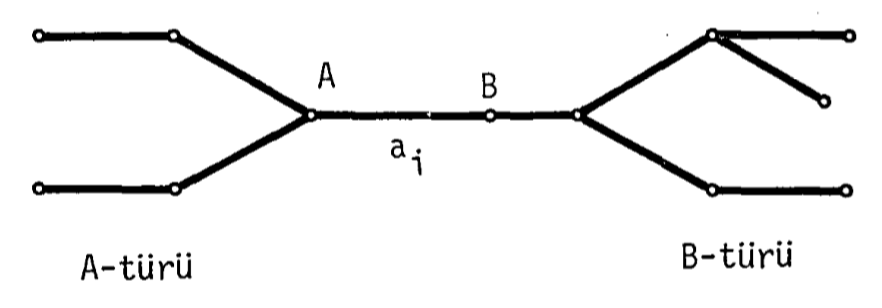
\includegraphics[width=0.65\textwidth]{images/4}
		\caption*{ Şekil 3.2.2 Çizgideki düğümlerin A ve B olarak iki kümeye ayrılması }
		\label{fig:Aa}
	\end{figure}

kümeye ayrılabilir (Şekil 3.2.3). $a_i$ nin tanımladığı t-kesitleme $K_i$,\\ \\
\hspace*{20ex}  $K_i  =  a_i  \bigcup  a_AB $\\ \\
dir. Ayrıca,\\
\begin{figure}[htb]
	\centering
	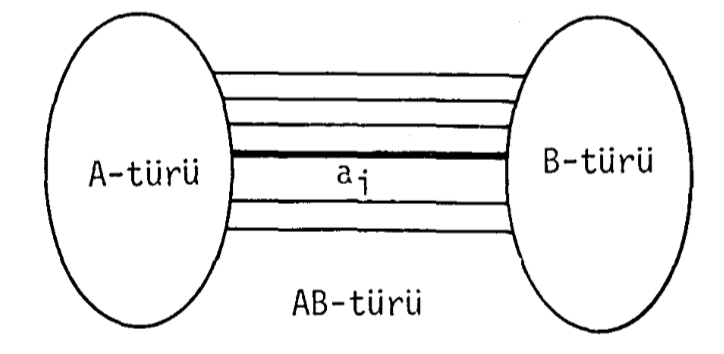
\includegraphics[width=0.65\textwidth]{images/5}
	\caption*{ Şekil 3.2.3 Çizgideki düğümlerin A, B, AB olarak  kümeye ayrılması }
	\label{fig:Bb}
\end{figure}
\end{document}